Hip\'otesis: El algoritmo genera el raiting de cada equipo en base a los raitings de los equipos contra los que jug\'o. Si un equipo no jug\'o contra nadie su rating es 1/2. Cuando el equipo A gana un juego, todos los dem\'as equipos a los que le gan\'o van a tener un mayor rating ya que A ahora gan\'o m\'as partidos y es m\'as valioso. Si un equipo B no jug\'o nunca contra ning\'un equipo que haya jugado con A, el resultado de un nuevo partido de A no debe afectar a B.

Para graficar y analizar la situaci\'on vamos a graficar a los equipos como nodos de un grafo, y cada partido ganado es una arista dirigida con sentido al equipo que perdi\'o.

Adem\'as, vamos a dividir a la hip\'otesis en partes. Primero analizamos que pasa cuando tenemos varios equipos (por ejemplo 5 como en la figura) corriendo la instancia correspondiente obtenemos que los 5 equipos tendr\'an rating igual a 1/2, como quer\'iamos ver.

\begin{figure}[h!]
  \begin{center}
	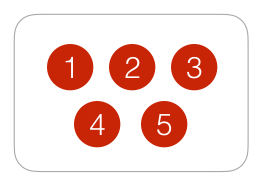
\includegraphics[scale=0.50]{imagenes/cualitative/fairness/fairness1.png}
	\caption{Equipos que no juegan nunca entre s\'i}
	\label{bChange}
  \end{center}
\end{figure}

Luego tomamos un grafo no conexo como el de la figura siguiente. Usando el CMM vemos que como dice la hip\'otesis, el rating de los equipos 1, 2, 3 y 4 no cambia al variar el resultado de los partidos entre el grafo conexo de 5, 6 y 7.

\begin{figure}[h!]
  \begin{center}
	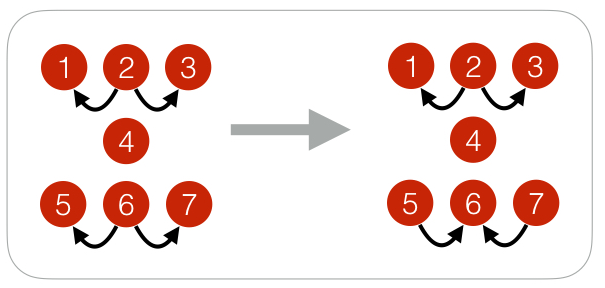
\includegraphics[scale=0.50]{imagenes/cualitative/fairness/fairness2.png}
	\caption{Modificaci\'on de resultado de partidos en subconjunto no conexo}
	\label{bChange}
  \end{center}
\end{figure}

Ahora que vimos que el resultado de un partido solo puede afectar a los nodos tales que existe un camino entre ellos, veamos el caso de un grafo conexo. Analizamos c\'omo afecta el resultado de un partido donde uno de los jugadores tanto gan\'o como perdi\'o contra otros equipos y queremos ver c\'omo afect\'o al rating de los otros equipos.
Antes de jugar el equipo 4 contra el 2 nos encontramos en una situaci\'on donde 2 tiene rating 1/2 y luego 1 es el que mayor rating tiene ya que le gano a 3 y a 4, luego 3 y 4 tienen mayor rating que 5, 6, 7 y 8.
En el caso de que 4 le gane a 2, podemos observar utilizando el CMM que el equipo 1 aumenta su rating, como enunciamos en la hip\'otesis. Esto se da ya que 4 tiene m\'as partidos ganados y es m\'as valioso ganarle a 4 ahora que antes. Adem\'as el equipo 2 disminuye su rating ya que antes no hab\'ia perdido y ahora s\'i. Pero lo extraño que observamos es que todos los equipos excepto el 2 aumentan su rating, incluso los que est\'an muy poco relacionados, como el equipo 5. Esto se da ya que el rating de cada equipo est\'a en relaci\'on al rating de los equipos contra los que jug\'o. Y al aumentar el rating de 4, aumenta el rating de 1 ya que 1 jug\'o contra 3 y contra 4. Por eso mismo aumenta el de 3, luego 5 y 6, etc.
Para el caso de que 4 pierde contra 2 observamos la misma situaci\'on solo que 2 ahora aumenta su rating y todo el grafo excluyendo al 2 lo disminuye.

Tambi\'en analizando los n\'umeros m\'as en detalle pudimos observar que la jugada entre 2 y 4 afecta en proporci\'on mucho mayor a los ratings de 2 y de 4 que al resto. De hecho cuantas m\'as aristas de distancia m\'as disminuye el impacto en el rating al punto de que el cambio en 5 y 6 es muy poco significativo.

\begin{figure}[h!]
  \begin{center}
	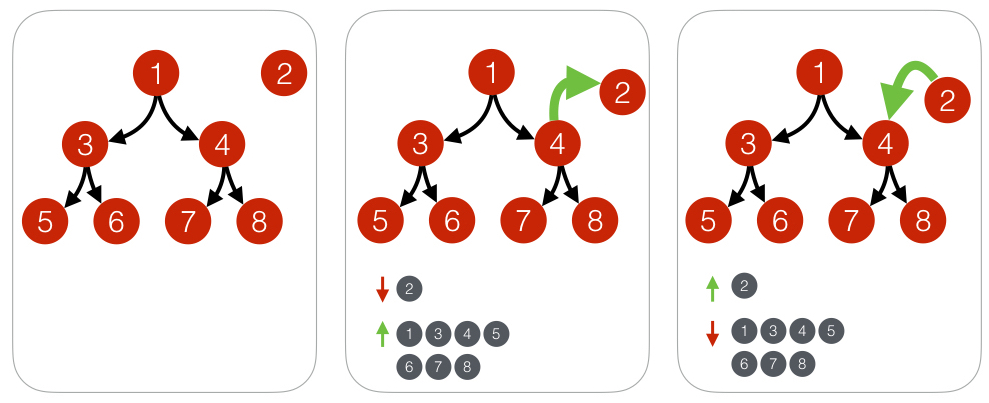
\includegraphics[scale=0.50]{imagenes/cualitative/fairness/fairness3.png}
	\caption{Modificaci\'on de raitings en base al resultado de un partido}
	\label{bChange}
  \end{center}
\end{figure}

Conclusiones: Aunque creemos que el CMM aporta mucho valor al lograr que ganarle a un equipo que gana mucho aumente m\'as el rating que ganarle a un equipo que gana poco, notamos comportamientos que no son quiz\'as tan intuitivos para establecer los resultados del juego. El hecho de que 4 le gane a 2 no luce tan claramente como justificaci\'on para que los equipos 7 y 8 (quienes nunca le ganaron a 4) aumenten su rating. De todos modos creemos que es una muy buena aproximaci\'on para un manejo m\'as real de los resultados de una competencia.

